%% Set up the geometry and hyperref packages
\geometry{
  a4paper,
  total={170mm,257mm},
  left=20mm,
  top=20mm,
}

\hypersetup{
    colorlinks=true,
    linkcolor=black,
    filecolor=magenta,
    urlcolor=cyan,
}

%% Define the cover page
\newcommand{\createcover}{
  \begin{titlepage}
    \centering
    
\includegraphics[width=0.3\textwidth]{logos/logo_FIB.png}\hspace{0.1cm}
    
\includegraphics[width=0.3\textwidth]{logos/logo_ETSETB.png}\hspace{0.1cm}
    
\includegraphics[width=0.25\textwidth]{logos/logo_FME.png}\\[1cm]
    
    {\large\bfseries BACHELOR'S DEGREE IN MATHEMATICS \\[0.3cm]  BACHELOR'S DEGREE IN DATA SCIENCE AND ENGINEERING}\\[1cm]
    
    {\huge\bfseries Automated detection of tumoural cells with graph neural networks}\\[1cm]

    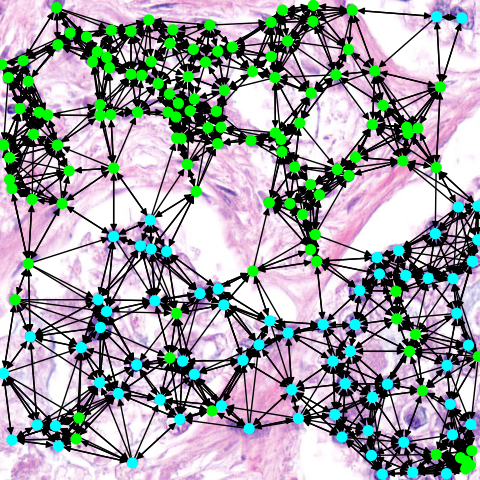
\includegraphics[width=0.7\textwidth]{imgs/graph_overlay.png}\\[2cm]
    
    {\large\itshape Author: Jose Pérez Cano}\\
    {\large\itshape Supervisor: Philippe Salembier Clairon}\\
    {\large\itshape Co-director: Ferran Marqués Acosta}\\[0.5cm]
    
    {\large June 2023}\\
    \vfill
    
\includegraphics[width=0.3\textwidth]{logos/logo_CFIS.jpg}
  \end{titlepage}
}

%% Define the abstract page
\newcommand{\createabstract}[4]{
\selectlanguage{#1}
\begin{abstract}
    \noindent #2 % Abstract text.
    \noindent \\
    \noindent #3 % Keywords.
    \noindent \\
    \noindent #4 % AMS codes
\end{abstract}
\selectlanguage{english}
}

%% Set up the headers and footers
\pagestyle{fancy} % Line on top of sections
\fancyhf{}
\renewcommand{\chaptermark}[1]{\markboth{#1}{}} 
\renewcommand{\sectionmark}[1]{\markright{\thesection\ #1}}
\fancyhead[L]{Jose Pérez Cano}
\fancyhead[R]{\leftmark}
\fancyfoot[C]{\thepage}
\fancypagestyle{plain}{
  \fancyhead{}
  \renewcommand{\headrulewidth}{0pt}
}

%% Customize the chapter and section formatting
\titleformat{\chapter}[display]
  {\normalfont\huge\bfseries}{\chaptertitlename\ \thechapter}{20pt}{\Huge}
\titlespacing*{\chapter}{0pt}{-30pt}{40pt}